\chapter{Implementation}
\label{chap:implementation}

% In diesem Kapitel beschreiben Sie Ihre Lösung des Problems. Geben Sie dem Leser genügend Einblick in die Lösung, so dass er Ihre Arbeit entsprechend würdigen kann. Verwenden Sie aber Anhänge für Dinge, die hier nicht unbedingt bis ins letzte Detail verstanden werden müssen.

\section{Komponenten/ Technologien}
\label{sec:komponenten}
Wie in der Aufgabenstellung erwähnt, sollte die Wissensmodellierung ursprünglich mit Hilfe von Apache Stanbol umgesetzt werden. Während der Arbeit wurde erkannt, dass diese Technologie, für die vorgesehene Aufgabe, nur bedingt nutzbar  ist. In Apache Stanbol ist es möglich die modellierte Wissensdomäne zu importieren. Das Modell wird als Ontologie in Form von Tripeln gespeichert. Die Objekte, deren Eigenschaften sowie Relationen lassen sich allerdings nicht direkt ansehen.

Um Fragen an die Wissensdatenbank stellen zu können, ist eine entsprechende Schnittstelle notwendig. Diese wird von Stanbol in Form eines SPARQL-Endpoints zur Verfügung gestellt. Der SPARQL-Endpoint nutzt jedoch die ContentHub-Komponente von Stanbol als Datenbasis und diese stellt nur gewonnenes Wissen durch angereicherte Inhalte, aufgrund von Ontologien und Regeln, zur Verfügung.

Nach einiger Recherche stellt sich heraus, dass es zwar möglich wäre mehr Datenquellen für den SPARQL-Endpoint zu nutzen, dies würde jedoch erheblichen Mehraufwand in Form einer eigenen Implementation bedeuten. Somit ist Stanbol für diese Arbeit nicht das geeignete Produkt.


\subsection{Stanford Protégé}
\label{subsec:protege}

Protégé ist eine Entwicklungsumgebung von OWL Ontologien. Es wurde von der Standford University entwickelt. Heute handelt es sich um  eines der bekanntesten OWL Editoren im Bereich der OWL Modellierung.
Protégé unterstützt sowohl die Modellierung der OWL Ontologie, wie auch das Reasoning mittels verschiedener Reasoner.


\subsubsection{Features}
\label{subsubsec:protege_features}

Protégé unterstützt die Entwicklung von OWL Ontologien. Die Ontologien können in unterschiedlichen Schreibweisen, wie zum Beispiel OWL/XML oder RDF/XML abgespeichert werden. Protégé erlaubt den Import und Export solcher OWL Dateien. Dabei können in einem Workspace mehrere Ontologien Verwendet werden. Die Entwicklungsumgebung bietet verschiedene Ansichten von der gleichen Ontologie an. \\
Neben dem Anlegen und bearbeiten einer Ontologie können in Protégé  swrl Regeln hinzugefügt werden. Diese werden von Protégé direkt in das owl File eingearbeitet. \\
Protégé bietet die Möglichkeit Anfragen mittels der Abfragesprache SPARQL abzusetzten. Ist einer der Reasoner gestartet unterstützt die Umgebung zusätzlich das Reasoning. Es können verschieden Reasoner wie zum Bespiel FACT ++ oder Pellet (siehe:~\ref{ssubsec:reasoner}) eingesetzt werden.\cite{protegeFeatures} 


\subsubsection{View}
\label{subsubsec:protege_view}

Die Benutzerfreundlichkeit von Protégé wird dadurch erreicht, dass eine Ontologie in verschiedenen Views dargestellt werden. So gibt es neben der Entity-View, welche sämtliche Elemente einer Ontologie enthält für jedes Elementtyp wie Klassen/ Dateneigenschaften oder Individuen eine eigene Ansicht.\\
Alle Ansichten sind als Baumstruktur organisiert. Dies bietet eine klare Übersicht und ermöglicht eine hierarchie getreue -Abbildung des dahinterliegenden XML Dokuments.\\ 
Neben der darstellung der im XML Dokument abgespeicherten Informationen bietet Protégé noch andere Ansichten. So kann der, aus der Ontologie entstehenden, Graphen in der View OntoGraf angesehen werden.\cite{protegeView}

Eine Nützliche Eigenschaft der Views ist, dass nach dem Starten eines Reasoners, die abgeleiteten Schlüsse direkt in der Hirarchie angezeigt werden.

\subsection{Clark \& Parsia Stardog}
\label{subsec:stardog}

Im laufe der Arbeit wurde festgestellt, dass das Reasoning unter Protégé nicht einwandfrei funktioniert, also sparql Anfragen nicht erwartungsgemäss beantwortet. Ausserdem exisitert in Protégé keine, mit einem sinnvollen Zeit und Arbeitsaufwand zu verwendende, http Schnittstelle. Aus diesen Gründen wird zur Weiterverarbeitung, der in Protégé erzeugten Ontologie Stardog verwendet.\\
Konkret wird unter Stardog eine Datenbank erstellt, in welche die vorbereitete Ontologie im RDF/XML Format eingespielt wird. Stardog bietet dann die Möglichkeit per http Anfragen über REST Anfragen zu stellen. Dabei ist ein komplettes und zuverlässiges Reasoning gewährleistet.

Bei Stardog handelt es sich um ein führendes Entwicklung und Anwendungssystem von Wissenmodellierung mit Suchen, Anfragen und Reasonings für Java Systeme. Stardog bietet unterschiedliche Formate an. Neben der kostenpflichtigen Enterprise Version, gibt es glücklicherweise eine Community Version. Diese bietet eine eingeschränkte Vielfallt von Datenbanken, Benutzern und Verbindungen, ist aber frei verfügbar.\cite{stardog}

Stardog kann auch als Graphische Datenbank bezeichnet werden. Dabei unterstützt es viele nützliche Verwendungsformen:
\begin{itemize}
	\item RDF Daten Modelle
	\item SPARQL\footnote{\url{http://www.w3.org/TR/sparql11-query/}} als Abfragesprache
	\item HTTP und SNARL Protokolle als remote Zugriff und Kontrolle
	\item OWL 2 zur Modellierung der Ontologien
	\item Regeln für Inferenz und Datenanalyse
	\item Java, JavaScript, Ruby, \.NET und weitere Programmiersprachen
\end{itemize}
\cite{stardogDocu}

\subsubsection{Features}
\label{ssubsec:features}
Der folgende Abschnitt basiert auf der offiziellen Stardog Dokumentation.\cite{stardogDocuUsing}\\

Querying:\\
Anfragen können auf einer RDF Datenbank mittel der SPARQL Abfragesprache gestellt werden. Mit dem folgenden Befehlt kann eine Afrage abgesetzt werden.\\
\begin{lstlisting}
		\$ stardog query <Datenbankname> ``<SPARQLAnfrage>''
\end{lstlisting}	
Neben sämtlichen SPARQL Funktionen Unterstützt Stardog weitere von XPath und SQRL.\ Einige dieser Funktionen können für Anfragen oder Regeln verwendet werden.

Updating:\\
Es gibt verschiedene Arten um in Stardog die Datenbank zu aktualisieren. Die üblichste Art ist das Updaten mittels CLI und SPARQL Queries. Diese Funktion wird in diesem Projekt nicht genutzt, da die Daten in Protégé aufbereitet werden.

Versioning:\\
Stardog unterstützt Versionierung mittels ``graph change management capability'', welche es dem Benutzer erlaubt Änderungen zu verfolgen.\\
Die Versionierung für eine Datenbank standarmässig deaktiviert und muss bei bedarf aktiviert werden.

Exportieren:\\
Es ist möglich die in der Stardog Datenbank enthaltenen Daten nach RDF zu exportieren. Insbesondere können auch nur einzelne ``named graph'' exportiert werden.

Searching:\\
Stardog includes an RDF-aware semantic search capability: it will index RDF literals and supports information retrieval-style queries over indexed data

Obfuscating:\\
When sharing sensitive RDF data with others, you might want to (selectively) obfuscate it so that sensitive bits are not present, but non-sensitive bits remain. For example, this feature can be used to submit Stardog bug reports using sensitive data.

% TODO: Frage: soll ich die ganzen Usings beschreiben? Ich bin insgesammt ein bisschen verwirrt. Herr Eckerle hat ja gesagt er will nur so blabla drin. Aber irgendwie hab ich das gefühl solche sachen müssen doch schon irgendwo rein?!
und was ist mit der ganzen Technik hinter Stardog? 
\subsubsection{Reasoner}
\label{ssubsec:reasoner}
Reasoner sind Komponenten, welche eine Folgerung von implizitem Wissen zulassen bzw.\ bieten. Es handelt es sich um eine Art ``Verstehen'' durch Maschinen. Man möchte also implizite Fakten finden, welche durch explizite Fakten in einer Ontologie definiert sind. 

Als Reasoner kommt Pellet zum Einsatz. Dabei handelt es sich um einen Reasoner, für die Sprache OWL-DL~\footnote{\url{http://www.w3.org/TR/owl-ref/\#OWLDL}}, welche wiederum eine Teilsprache von OWL darstellt. Eine komplette Unterstützung des OWL full Profils ist so nicht möglich, da dieses nicht entscheidbar ist, daher beschränkt sich die Umsetzung auf OWL DL\@. Pellet setzt dabei komplett die Spezifikation der WebOnt Arbeitsgruppe um. OWL-DL ist eine syntaktische Variante der Beschreibungslogik SHOIN (D).

\begin{figure}[htbp]
\centering \rotatebox{0}{\scalebox{0.5}[0.5]{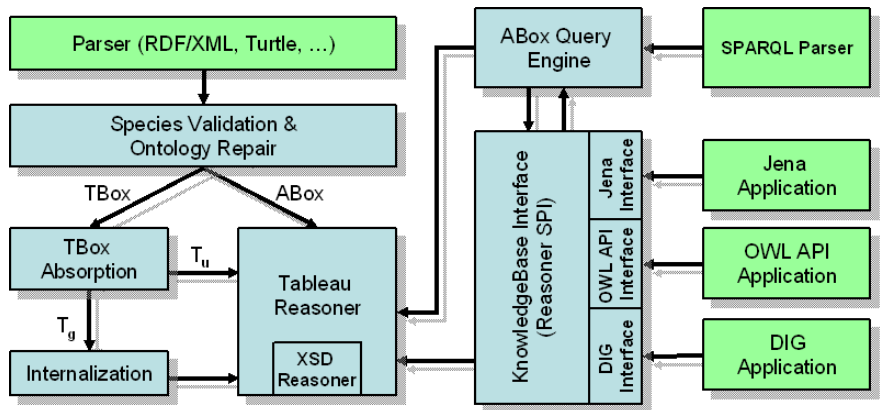
\includegraphics{bilder/pellet_komponenten.png}}}
\caption{Hauptkomponenten des Pellet-Reasoners.\label{fig:pellet_komponenten}\protect\footnotemark}
\end{figure}
\footnotetext{\cite[S. 6]{sirin:pellet05}}

\subsubsection{Beschreibungslogik}
\label{subsubsection:beschreibungslogik}
Beschreibungslogiken sind Formalismen um Wissen darzustellen, dabei sind sie eine Teilmenge der Prädikatenlogik. Sie stellen den Kern von Wissensrepräsentationssystemen dar, in dem sie eine Struktur für eine Wissensbasis und den damit verbundenen Methoden zur Folgerung bieten (vgl.~\cite{dl:baader2003}).

Die Struktur, welche Beschreibungslogiken als Wissensbasis bereitstellen, besteht aus einem Schema (Tbox, Regeln), sowie aus den Daten (Abox, Fakten).

Die Semantik von Beschreibungslogiken wird durch Interpretationen definiert:

\noindent\hspace*{16mm} $ I = (\Delta^I, \cdot^I) $

Dabei ist:
\begin{itemize}
\item $ \Delta^I $

    Die (Wissens-) Domäne (eine nicht leere Menge).

\item $ \cdot^I $

    Eine Funktion zur Interpretation von:
    \begin{itemize}
        \item Konzepten (Klassen, A)

            Wobei $ A^I $ eine Teilmenge von $ \Delta^I $ ist.
        \item Rollen (Eigenschaften, R)

            Wobei $ R^I $ eine binäre Relation auf $ \Delta^I $ ist.
        \item Individuen (i)

            Wobei $ i^I $ Element von $ \Delta^I $ ist.
    \end{itemize}
\end{itemize}

Die Funktion zur (Wissens-) Interpretation $ \cdot^I $ definiert, wie atomare Konzpte, Eigenschaften und Individuen zu interpretieren sind. Eine Interpretation, welche allen Axiomen einer Ontologie in Beschreibungslogik genügt ist ein Modell der Ontologie.

Eine Ontologie in Beschreibungslogik ist eine Menge von Termen und deren Relationen. Die Interpretation dieser Ontologie stellt als ein Modell dar, welches die Ontologie abbildet.

Die Pellet zu Grunde liegende Beschreibungslogik SHOIN (D) ist ein Kürzel und steht für:
\begin{itemize}
\item \textit{S}

ALC (Attributive Concept Language with Complements) mit einer transitiven Rolle. Bei ALC handelt es sich um die kleinste Beschreibungslogik, welche aussagenlogisch geschlossen ist (d.h.\ sie bietet, entweder implizit oder explizit, Konjunktion, Union und Negation von Klassen (-beschreibungen)). Eine Rolle entspricht einer Eigenschaft bzw.\ einem Prädikat in der Prädikatenlogik erster Stufe.

\item \textit{H}

    Rollenhierarchie (Sub-Eigenschaften), z.B. rdfs:subPropertyOf.

\item \textit{O}

    Nominal, z.B. Wochenden = {Samstag, Sonntag}.


\item \textit{I}

    Inverse Rolle (inverse Eigenschaft bzw.\ Prädikt).

\item \textit{N}

    Nummerische Einschränkung, z.B. >= hatKind 1.

\item \textit{(D)}

    Nutzung von Wertebereichen, Werten oder Datentypen.
\end{itemize}

(vgl.~\cite{dl:baader2003})

\subsubsection{Folgerung}
\label{subsubsection:folgerung}
Die W3C Spezifikation betreffend der Umsetzung eines Reasoners definiert zwei Arten von OWL Dokumentprüfungen: Prüfung auf korrekte Syntax sowie Prüfung der Konsistenz. Bei der Konsistenzprüfung geht es darum festzustellen, ob eine gegebene Eingabe anhand einer definierten Spezifikation syntaktisch korrekt ist. Jedoch macht eine reine Umsetzung der genannten Prüfungen wenig Sinn. Man möchte ja eine Ontologie möglichst effektiv nutzen können, zum Beispiel um indirektes Wissen abzuleiten.  Da OWL DL eine syntaktische Variante der Beschreibungslogik SHOIN (D) darstellt, liegt es nahe, mittels einem Reasoner folgende Methoden zur Inferenz zur Verfügung zu stellen:
\begin{itemize}
\item \textit{Konsistenzprüfung}

Stellt sicher, dass sich in der Ontologie keine gegenstätzlichen Fakten befinden. Konkret bedeutet dies anhand der OWL Semantik~\footnote{http://www.w3.org/TR/owl-semantics/}, dass die Konsistenz einer ABox in Bezug auf eine TBox geprüft wird.
\item \textit{Konzept-Erfüllbarkeit}

Stellt sicher, dass Objekte einer Klasse instanziert werden können. Ist dies nicht der Fall, so ist die Ontologie inkonsistent.
\item \textit{Klassifikation}

Berechnet die Relationen zwischen Subklassen, stellt also die Klassenhierarchie auf. Dies ermöglicht das Abfragen der Ontologie.
\item \textit{Gewinnung von Erkenntnissen}

Findet die spezifischste Klasse eines Objektes, leitet also den direkten Typ jedes Objektes ab.
\end{itemize}
(vgl. \citet[S. 1 und 2]{sirin:pellet05})

Bei der eigentliche Komponente, welche in Pellet zur Folgerung eingesetzt wird, handelt es sich um den Tableau Reasoner, welcher den gleichnamigen Algorithmus verwendet. Dieser reduziert ein Problem der Folgerung auf ein Problem der Konzept-Erfüllbarkeit, wobei er eine Interpretation sucht, welche die gefragten Konzepte erfüllt. Solch eine Interpretation wird inkrementell als eine Art Tafel (eben, Tableau) aufgebaut.

Nachfolgend ein Beispiel, gegeben sei:
$ Prolog \subseteq LogischeProgrammiersprache, LogischeProgrammiersprache \subseteq Programmiersprache $
Man stellt nun folgende Anfrage:
$ if Prolog \subseteq Programmiersprache $

Der Prozess der Folgerung findet nun wie folgt statt:
\begin{itemize}
    \item Testen, ob ein Individuum existiert, welches eine logische Programmiersprache, aber keine Programmiersprache ist. Man möchte also die Erfüllbarkeit des Konzeptes $ C_0 = (Prolog \sqcap \neg Programmiersprache) $ testen.
    \item $ C_0(x) \Rightarrow Prolog(x), (\neg Programmiersprache)(x) $
    \item $ Prolog(x) \Rightarrow LogischeProgrammiersprache(x) $
    \item $ LogischeProgrammiersprache(x) \Rightarrow Programmiersprache(x) $
        $ \Rightarrow $ Konflikt!
\end{itemize}
Wie ersichtlich ist, ist das Konzept $ C_0 $ nicht erfüllbar, die Anfrage $ Prolog \subseteq Programmiersprache $ trifft also innerhalb der gegebenen Ontologie zu. Der Beweis wird mittels Kontradiktion erbracht.

Der generelle Prozess der Folgerung läuft wie folgt ab:
\begin{itemize}
    \item Umwandlung eines Konzeptes bzw.\ der Konzepte in die negierte Normalform (NNF), die Negation $ \neg $ befindet sich vor Konzeptnamen.
    \item Ablegen des umgewandelten Konzeptes als $ C_0 $.

        Der Algorithmus hat also die Datenbasis (Abox) $ A_0 = {C_0(x_0)} $
    \item Regeln zur Transformation auf die Datenbasis (Abox) so weit als möglich anwenden.
    \item Wurde eine gültige Datenbasis (Abox) gefunden, so ist $ C_0 $ erfüllbar.
    \item Wurde keine gültige Datenbasis unter Berücksichtigung aller (Such-) Pfade gefunden, so ist $ C_0 $ nicht erfüllbar.
\end{itemize} (vgl.~\cite{horrocks2002} und~\cite{horrocks2005})
